%\documentstyle[epsf,twocolumn]{jarticle}       %LaTeX2e仕様
%\documentclass[twocolumn]{jarticle}     %pLaTeX2e仕様(platex.exeの場合)
\documentclass[twocolumn]{ujarticle}   %pLaTeX2e仕様(uplatex.exeの場合)
%%%%%%%%%%%%%%%%%%%%%%%%%%%%%%%%%%%%%%%%%%%%%%%%%%%%%%%%%%%%%%
%%
%%  基本バージョン
%%
%%%%%%%%%%%%%%%%%%%%%%%%%%%%%%%%%%%%%%%%%%%%%%%%%%%%%%%%%%%%%%%%
\setlength{\topmargin}{-45pt}
%\setlength{\oddsidemargin}{0cm}
\setlength{\oddsidemargin}{-7.5mm}
%\setlength{\evensidemargin}{0cm}
\setlength{\textheight}{24.1cm}
%setlength{\textheight}{25cm}
\setlength{\textwidth}{17.4cm}
%\setlength{\textwidth}{172mm}
\setlength{\columnsep}{11mm}

%\kanjiskip=.07zw plus.5pt minus.5pt


% 【節が変わるごとに (1.1)(1.2) … (2.1)(2.2) と数式番号をつけるとき】
%\makeatletter
%\renewcommand{\theequation}{%
%\thesection.\arabic{equation}} %\@addtoreset{equation}{section}
%\makeatother

%\renewcommand{\arraystretch}{0.95} 行間の設定
%%%%%%%%%%%%%%%%%%%%%%%%%%%%%%%%%%%%%%%%%%%%%%%%%%%%%%%%
%\usepackage{graphicx}   %pLaTeX2e仕様(\documentstyle ->\documentclass)
\usepackage[dvipdfmx]{graphicx}
\usepackage{subcaption}
\usepackage{multirow}
\usepackage{amsmath}
\usepackage{url}
%%%%%%%%%%%%%%%%%%%%%%%%%%%%%%%%%%%%%%%%%%%%%%%%%%%%%%%%
\begin{document}

	%bibtex用の設定
	%\bibliographystyle{ujarticle}
	\twocolumn[
	\noindent

	\hspace{1em}
	2020 年 04 月 10 日
	ゼミ資料
	\hfill
	M2 寺内 光

	\vspace{2mm}

	\hrule

	\begin{center}
		{\Large \bf 進捗報告}
	\end{center}


	\hrule
	\vspace{3mm}
	]

	% ‚ここから 文章 Start!
	\section{今週やったこと}
	AutoML 周りの基本的な背景等のリサーチをした.全体像としての AutoML を俯瞰するなら \cite{auto-ml} がよくまとまっていた.今週はリサーチした内容をメモ書き程度にまとめた.論文内引用等割愛しているので引用は \cite{automl-sota} を参考のこと.

	\section{AutoMLの大枠}
	\subsection{AutoMLのモチベーション}
	\cite{automl-sota} 近年深層学習で画像分類,画像検出,言語モデルなど様々なタスクが解かれているが,それらはいずれも伝統的に良いと信じられている方法や専門家の試行錯誤の末にデザインされたモデルを使用してきた.モデルは 100 万以上のパラメータを持ち,メモリを 500MB 以上も占有,モデル全体を通した浮動小数点操作は 15.3 億回にも達する.これは専門家でさえ十分なパフォーマンスを生み出すモデルを作成するのにかなりの時間とコストが必要であることを意味する.AutoML はこの厄介な開発コストを削減するためにデータの特徴量抽出,ハイパーパラメータ探索,ネットワークアーキテクチャといった機械学習の全体的なパイプラインを自動化するために生まれた概念である.図 \ref{fig:procedure}, \ref{fig:automl-overview} に AutoML の基本的な手続きを示す.各手続きの詳細は引用を参考.

	\begin{figure}[htb]
		\centering
		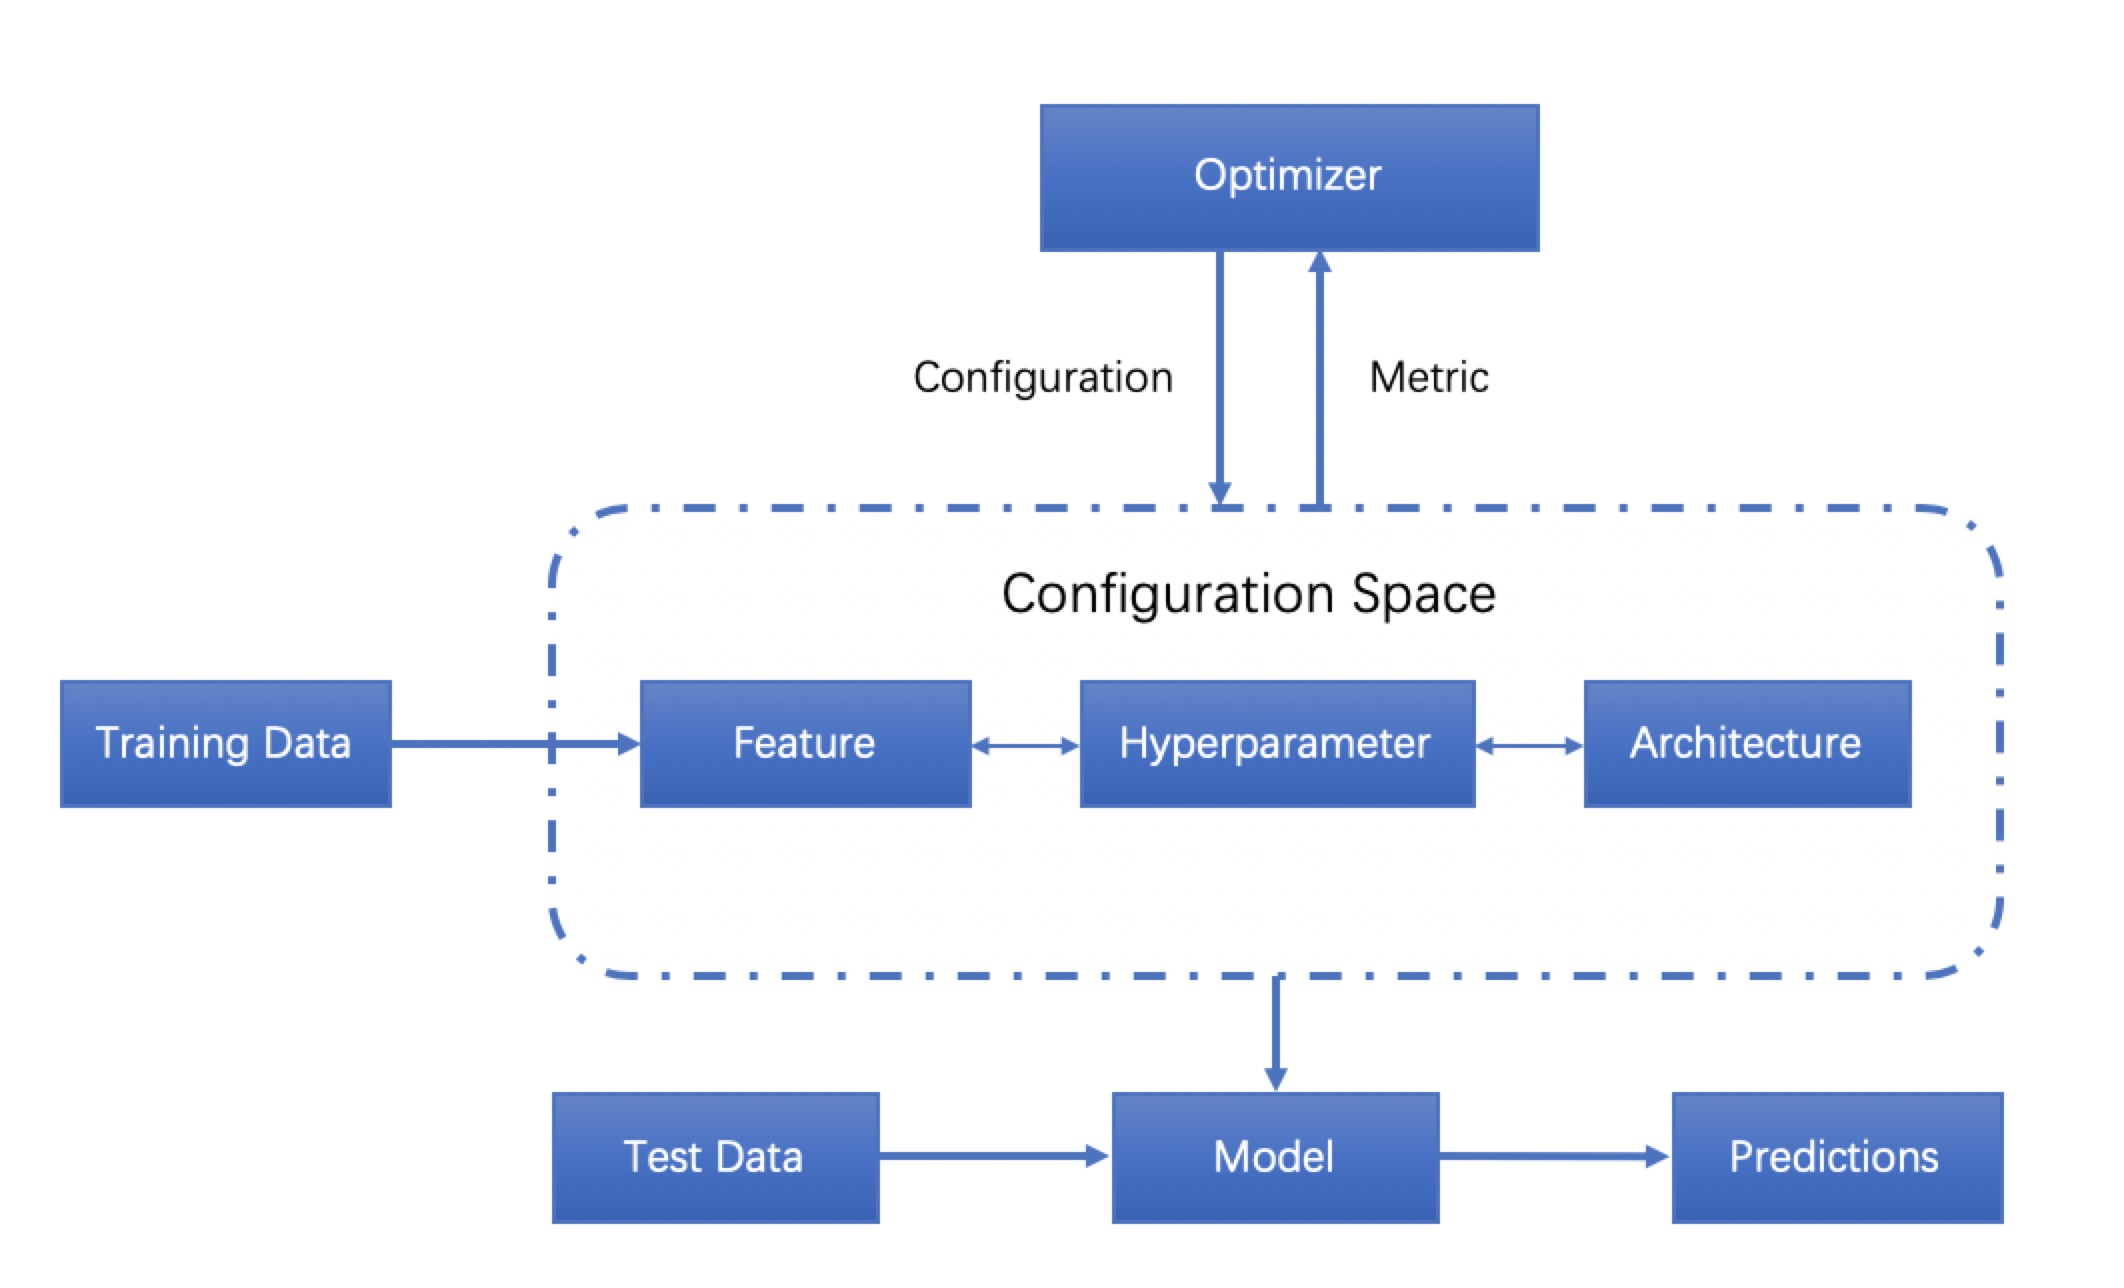
\includegraphics[width=1.0\columnwidth]{data/procedure.jpg}
		\caption{AutoML 全体図1}
		\label{fig:procedure}
	\end{figure}

	\begin{figure*}[htb]
		\centering
		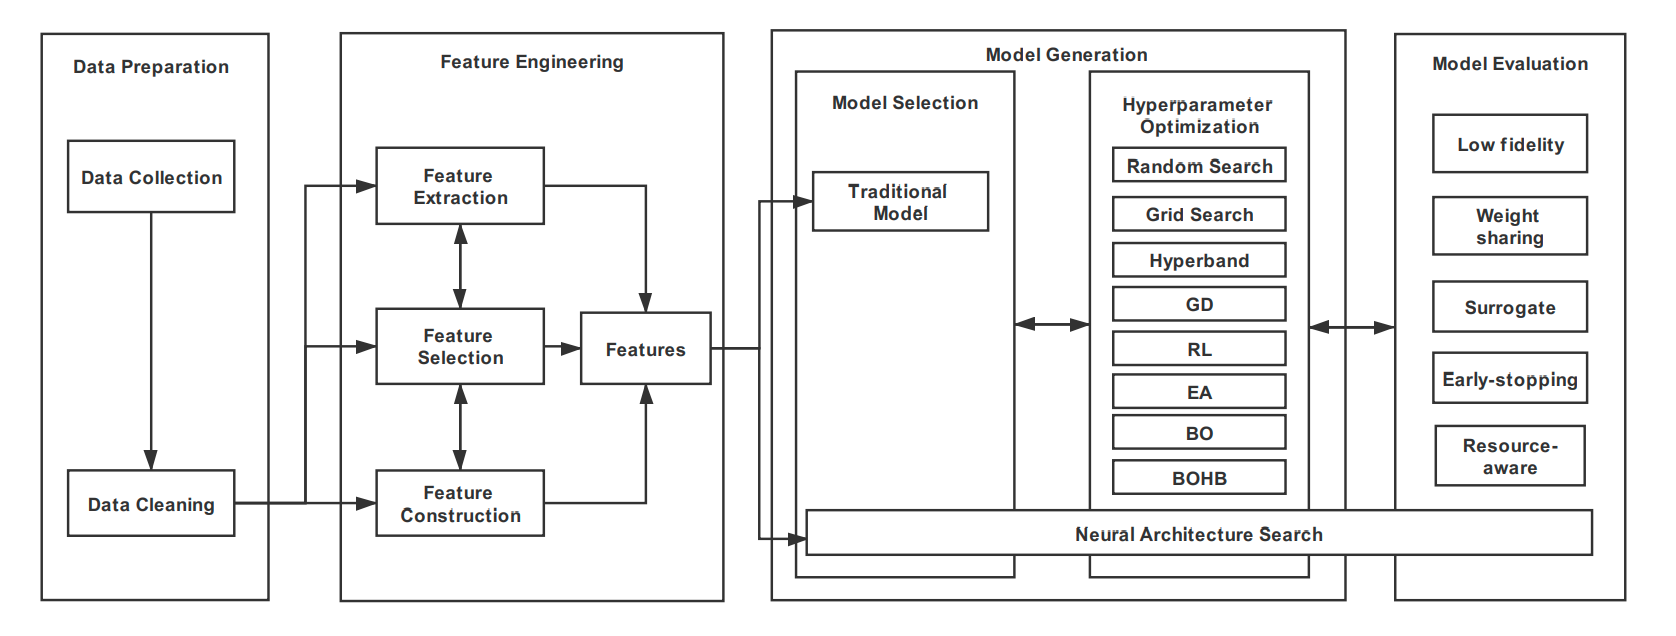
\includegraphics[width=2.0\columnwidth]{data/autoML-overview.png}
		\caption{AutoML 全体図2}
		\label{fig:automl-overview}
	\end{figure*}


	\subsection{AutoMLの種類}
	図 \ref{fig:automl-overview} で挙げたように,AutoML には Data Preparation,Feature Engineering, Model Generation, Model Evaluation のような段階がある.その中でも
	AutoMLの最も関心が持たれているトピックに Neural Architecture Search(NAS)があり,NAS においては Model Generation, Model Evaluation の段階についての自動最適化をする.
	NAS は以下の2つのタイプに分かれる.

	\begin{itemize}
		\item{model structure type}
		\item{model structure design by hyperparameter optimization(HPO)}
	\end{itemize}

	\subsubsection{model structure type}
	model structure type はネットワーク構造そのものを最適化する NAS の 1 種である.その種類に entire structures, cell-based structures, progressive structures, morphism-based structures などがある.

	entire structure type では,モデル構造全体の最適化をする.予め決められたノード数のブロックを用意し,そのブロックにおける演算が定義されている中で,そのブロック同士の連結関係などを最適化する.entire structure は モデル構造探索方法の最も直感的なタイプであるが,モデルが深くなればなるほど計算コストが膨大なものとなることや,小さいデータセットによって最適化されたモデルが大きな実データセットに適さないというような問題がある.

	 cell-based structure は従来の人間がデザインした良いモデルの構造から着想を得た手法のタイプであり,モデルをいくつかのセル構造に分割する.セルは複数の操作をまとめた構造を持っている.cell-base structure タイプは entire structure と異なり,大きなモデルでもセルの積み重ねによって簡単に構築することができる.そのため,例えばまず小さなデータセットで学習した後に,そのモデルを転移学習の手法で大きなデータセットの学習に用いることができる.全体として考えられる構造の組み合わせ数のオーダーとかの議論ものっているので興味がある人は引用を参考.cell-based structure は entire structure よりも効率的ではあるが,いくつかの欠点もあり,1 つにセルに含まれるブロック数 $B$ を予め決める必要があり,その $B$ が人の手で決める新たなハイパーパラメータとなってしまう点や,GPU メモリの制限によって浅いネットワークで探索を行わなければならず,探索空間と評価空間の乖離が起きてしまう点などが問題点として挙げられる.

	 progressive structure では上記の問題を解決するべく,階層型遺伝的表現を持った手法を提案しており,高いレベルのセルは低いレベルのセルを組み込むことで反復的に生成されるという特徴を持つ.上位レベルのセルを学習可能な隣接上三角行列によって表現することで,cell-based よりもより複雑で柔軟なトポロジ構造を構成することができる.また,progressive structure においては探索プロセスを複数の段階に分け,ネットワークの深さを段階ごとに深くしていくことで探索空間と評価空間の乖離問題を解消している.

	 morphism-based structure では上記と異なるアプローチをとっており, 「あるモデルを変換関数(IdMorphと呼ばれている)によってより深い, 広い等価なモデルに変換する」ことを目指す.この IdMorph は本来深さ方向と幅方向を別々に変換することしかできなかった.そこでこの手法の改善策として network morphism と呼ばれるネットワーク構造が生まれ, network morphism では親のネットワーク構造を子のネットワーク構造が継承することでより短く,強力なネットワーク構造を手に入れることを可能にした.network morphism は非恒等層を埋め込み,任意の非線形な活性化関数を処理することができる点や,深さ方向と幅方向およびカーネルの変換を1度の操作でできる点などが利点であるとされている.また先行研究によると,この morphism なアプローチによって畳み込み層を任意のニューラルネットワークモジュールに置き換えたり,ベイズ最適化の過程を NAS によって効率的に処理したりすることがを可能であると示されている.

	\subsubsection{HPO for NAS}
	HPO はネットワークのハイパーパラメータを最適化するタスクである.NAS によって HPO をする場合,その種類に reinforcement learning, evolution-based algorithm, gradient descent, Bayesian optimization などがある.

	reinforcement learning においては,エージェントは RNN にとって実装されており,各時刻 $t$ において探索空間から新たなアーキテクチャをサンプルするために 行動 $A_{t}$ を実行する.そして,新たな状態 $S_{t}$ および 報酬 $R_{t}$(ニューラルネットワークにおける訓練,評価識別率等) を観測し,エージェントのサンプリング戦略を決定する.このような reinforcement learning における HPO 戦略は CIFER-10 や Penn Treebank(PTB) データセットなどで最先端の結果を出したが,実行時間および計算資源のコストが多いという難点もあった.

	evolution-based algorithm は一般的な母集団ベースのメタヒューリスティックな最適化アルゴリズムであり,生物の進化に着想を得ている.evolution-based algorithm は 従来の最適化手法に比べ,高いロバスト性と広い適用可能性を持つアルゴリズムである.これをニューラルネットに適用するとした際,エンコーディング手法には直接的な方法と間接的な方法の大きく 2 つが存在する.例えば直接的な方法ではバイナリエンコーディングという手法を用い,ネットワークをグラフとみなした際,ノードが繋がれていれば 1 を立て,繋がれていなければ 0 を立てるという表現方法を用いている.この方法は単純であり,かつ計算コストを削減できるという点が強みである.より柔軟で様々な長さのネットワーク構造を表す手法として,ニューラルネットワークを非巡回有向グラフ(DAG)として扱う方法も存在する.また,間接的な表現方法の例としてはニューラルネットワークをラベル付きの木のセットとして扱う方法や,morphism 操作に基づく関数を用いた方法などがあり,これらの方法ではネットワークの生成方法を定義し,よりコンパクトな表現が可能となっている.

	gradient descent では上記のような離散的なサンプル方法に対し,ソフトマックス関数のような関数を用いて探索空間を連続的に探索する.gradient descent を用いた方法では,構造パラメータ $\alpha$ およびモデルパラメータ $\theta$ の結合最適化問題を解く.このような 2 段階最適化問題を解くためには訓練および評価データセットを用いてそれぞれを訓練する.詳細は引用を参考.この手法を用いた DARTS は探索時間を大きく削減したが,いくつかの問題点もあった.1 つめが操作の数に応じて線形的に必要な GPU メモリが増えることであり,この問題は探索空間を one-hot 形式でエンコードし,ネットワークのパスを制限するや,新しいパスの枝刈り手法によって緩和された.2 つめの問題はスキップ構造が後の探索段階で支配的な影響を与え,ネットワークが浅くなることでパフォーマンスが著しく低下することであった.この問題の緩和のためには通常のセルで 2 以上のスキップ構造を持つ場合などに追加の early stopping 基準を設けることや訓練および評価中に発生するスキップ接続操作の比率をドロップアウトによって調整することによる探索空間の正則化などがなされた.

	Grid Search,Random Search,evolution-based algorithm は独立試行であり,明らかに悪いパフォーマンスを持つ領域に対して何度もテストをすることになる.Bayesian optimization はその問題を解決する最適化手法である.Bayesian optimization では目的関数の確率モデルを構築し,最も有望なハイパーパラメータを選択し,最終的に真の目的関数により評価をする.つまり,Bayesian optimization では過去の評価結果を記録しておくことで確率モデルを繰り返し更新でき,その確率モデルはハイパーパラメータを目的関数のスコア確率に数学的にマッピングすることができる.Sequential model-based optimization (SMBO) は Bayesian optimization の簡潔な形式であり,最初に確率モデルを探索空間から小さくサンプリングすることで初期化する.その後,モデル $M$ は予め決められた取得関数に基づき選択された確率分布に従う新たなハイパーパラメータが設定されることで,データセット $D$ にフィッティングされていく.取得関数には improvement-based policies,improvement-based policies,improvement-based policies,portfolios of acquisition functions などがある.
	Bayesian optimization は持つ確率モデルによって Gaussian Processes,Tree Parzen
  Estimators (TPE),Random Forests など 3 つのカテゴリーに分かれる.Bayesian optimization は目的関数が確率的,非凸,または非連続であっても効果的である点が特徴的である.しかしながら,Bayesian optimization を DNN に適用するのはより困難であり,上記のような Hyperband(このあたり詳しく見れてない) と呼ばれるアルゴリズムは限られた計算資源のもとで有望なパラメータを見つけることができるが,最適な構成にはすばやく収束しないという難点もある.この問題はサイズが徐々に増加するサブデータセットで生成モデルをトレーニングすることによって緩和され,この改善によって探索の収束が 10 から 100 倍早くなったと検証されている.

	\section{現状の課題}
	\begin{itemize}
		\item{データ収集の自動化}
		\item{特定の操作やハイパーパラメータが他よりよい精度を出すことの科学的根拠の不足}
		\item{実験の再現性の困難}
		\item{畳み込みやプーリングなど従来の操作をベースとしたデザインによる柔軟性の欠如}
		\item{画像識別だけではない,より広い領域への NAS の適用}
		\item{古いデータを記憶しながら新しいデータで学習を行うためのメタ学習の導入}
	\end{itemize}

	等.

	\section{来週の予定}\noindent
	要相談.論文を書くなら今のままのマッチング問題の内容だと難しいような気もしている.

	\bibliographystyle{unsrt}
	\bibliography{2020_04_10_terauchi}

\end{document}
